\documentclass[nochap]{apuntes}

\usepackage{listings}
\usepackage{multirow}
\title{Memoria de la práctica 3}
\author{Guillermo Julián y Víctor de Juan}
\date{20/11/2013}

\begin{document}

\pagestyle{plain}
\maketitle

\section*{Ejercicio 0}

\begin{table}[htbp]
\centering
\begin{tabular}{|c|l|l|}
\hline \textbf{Tipo caché} & \textbf{Parámetro} & \textbf{Valor}  \\ 
\hline \multirow{3}{*}{\textbf{L1 Inst.}} 	& Tamaño  			& 32 KB  \\ 
\cline{2-3}  								& Asociatividad 	& 4  \\ 
\cline{2-3}  								& Tamaño de bloque  & 32 B  \\ 
\hline \multirow{3}{*}{\textbf{L1 Datos}} 	& Tamaño  			& 32 KB  \\ 
\cline{2-3}  								& Asociatividad 	& 8  \\ 
\cline{2-3}  								& Tamaño de bloque  & 64 B  \\ 
\hline \multirow{3}{*}{\textbf{L2}}		 	& Tamaño  			& 256 KB  \\ 
\cline{2-3}  								& Asociatividad 	& 8  \\ 
\cline{2-3}  								& Tamaño de bloque  & 64 B  \\ 
\hline \multirow{3}{*}{\textbf{L3}}		 	& Tamaño  			& 4 MB  \\ 
\cline{2-3}  								& Asociatividad 	& 16 \\ 
\cline{2-3}  								& Tamaño de bloque  & 64 B  \\ 
\hline 
\end{tabular} 
\caption{Tamaños de caché en los sistemas Linux de los laboratorios}
\end{table}

Sólo hay separación de datos entre caché e instrucciones en el nivel 1 de caché. Además, todas las cachés son asociativas de $n$ vías, 4 en el caso de la de instrucciones de nivel 1, 8 en las de datos de nivel y en la de nivel 2, y de 16 vías en la de nivel 3.

\section*{Ejercicio 1}

Esta es la gráfica generada con el script \texttt{genData}, que ejecuta los programas \texttt{slow} y \texttt{fast} guardando los tiempos de ejecución en un fichero (data/ej1/results)

\begin{center}
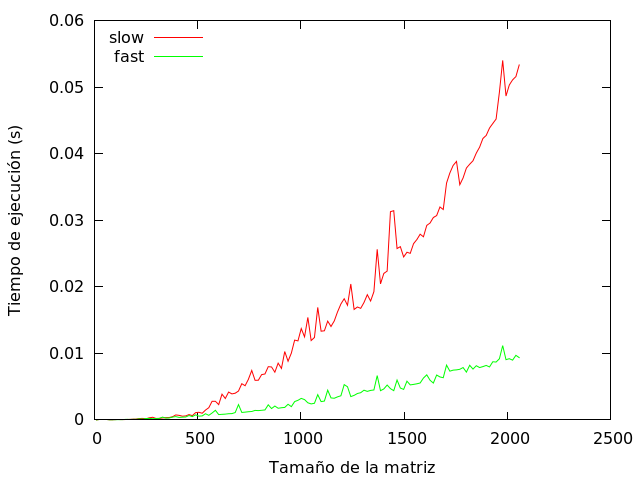
\includegraphics[width=0.7\textwidth]{graficas/fotos/ejercicio1.png}
\end{center}

Podemos comprobar claramente que el programa \texttt{slow} es más lento que el \texttt{fast}.

Examinando el código fuente vemos que el bucle de \texttt{fast} es:

\begin{lstlisting}[language=c]
for(i=0;i<n;i++)
	for(j=0;j<n;j++)
		sum += matrix[i][j];
\end{lstlisting}
y el código fuente de \texttt{slow} es:

\begin{lstlisting}[language=c]
for(i=0;i<n;i++)
	for(j=0;j<n;j++)
		sum += matrix[j][i];
\end{lstlisting}

Aquí se encuentra la única diferencia existente en el código, la indexación de las matrices. En \texttt{fast} se recorre por filas y en \texttt{slow} por columnas.

Otro factor importante es la reserva de memoria. Al reservarse memoria en 2 bloques, todas las filas de la matriz se encontrarán una seguida de otra en la memoria.

Gracias a estos 2 factores podemos explicar la diferencia de tiempos de ejecución vista en las gráficas.

Esto se debe al principio de proximidad de los datos de la caché. Por cómo está reservada la memoria, cada fila está almacenada probablemente en un mismo bloque (y sino en bloques contiguos) que se guarda en la caché cada vez que se referencia un elemento del bloque, de tal manera que podemos tener la fila entera en la caché. Si recorremos la matriz fila a fila nos aprovechamos de este principio consiguiendo una mayor utilización productiva de la caché. En cambio, si recorremos la matriz columna a columna, es muy probable que el elemento referenciado no se encuentre en el mismo bloque que el siguiente, de tal manera que en la mayoría de las lecturas se produce un fallo de caché porque los bloques guardados contienen los elementos de la misma fila y no de las columnas siguientes.

Esta hipótesis la contrasta el ejercicio 2, en el que comprobamos la diferencia de los fallos de caché.

\section*{Ejercicio 2}

Aquí presentamos las 4 gráficas asociadas a los 4 tamaños pedidos. Piden utilizar el número de pareja, pero \emph{cachegrind} necesita múltiplos de 2 en los tamaños de las cachés, asíque, aunque somos la pareja 10, hemos utilizado de número de pareja el 8 (el más cercano a nuestro número real, el 10).

Los datos han sido generados con el script genDataCaché, que va ejecutando \emph{slow} y \emph{fast} simulando con cachegrind distintos tamaños de caché. Los datos se almacenan en ficheros de la forma tamCache\_tamaño.dat en el directorio data. 

Después hemos generado los scripts de \texttt{gnuplot} con \texttt{genDataCache.sh}, para generar un script gnuplot por cada tamaño de la caché.

En todos los casos los fallos de escritura en caché son los mismo (en la gráfica no se aprecia pero en los ficheros de datos se ve claramente), pero los fallos de lectura de caché si son muy distintos, corroborando la hipótesis del ejercicio 1, que la diferencia de tiempos de ejecución la provocan los fallos de caché.

\subsection*{Gr\'aficas}
Las 4 gráficas generadas son:

\subsubsection*{8192 bytes}
Para una caché de tamaño $P*1024 = 8192$ bytes, con $P=8$ por ser el número de pareja potencia de 2 más cercano a nuestro número de pareja real (10).

\begin{center}
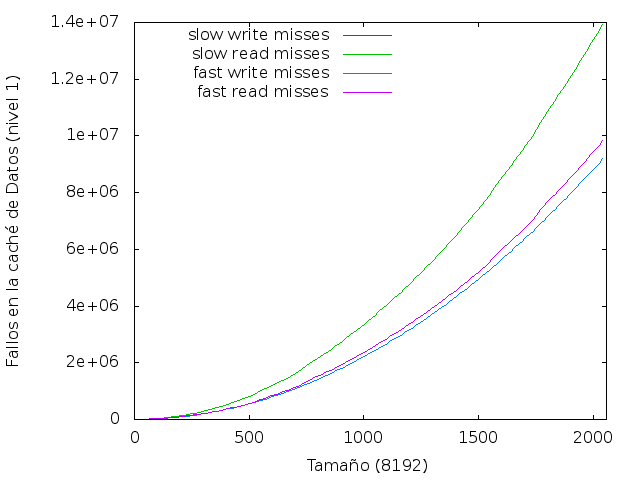
\includegraphics[width=0.8\textwidth]{graficas/fotos/Cache_8192.png}
\end{center}

Esta gráfica ha sido generada con el script de gnuplot \emph{graficas/tamCache\_8192.gp} a partir de los datos almacenados en \emph{data/ej2/tamCache\_8192.dat}
\subsubsection*{2*8192 bytes}
Para una caché de tamaño $P*2*1024$ bytes $= 16384 $ bytes.

\begin{center}
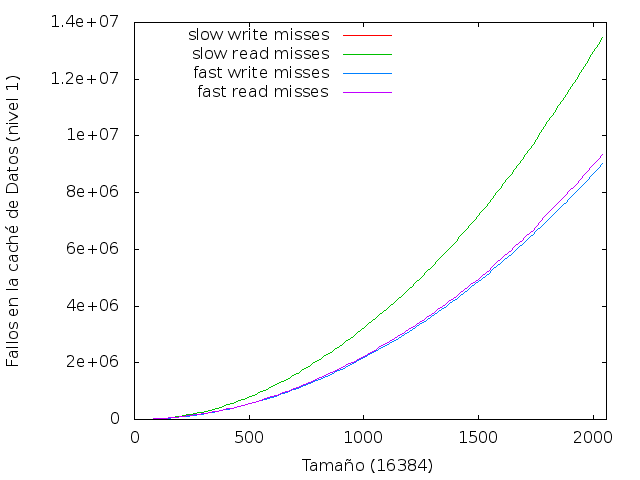
\includegraphics[width=0.8\textwidth]{graficas/fotos/Cache_16384.png}
\end{center}

Esta gráfica ha sido generada con el script de gnuplot \emph{graficas/tamCache\_16384.gp} a partir de los datos almacenados en \emph{data/ej2/tamCache\_16384.dat}

\subsubsection*{4*8192 bytes}

Para una caché de tamaño $P*3*1024\text{ bytes} = 32768 $ bytes.
\begin{center}
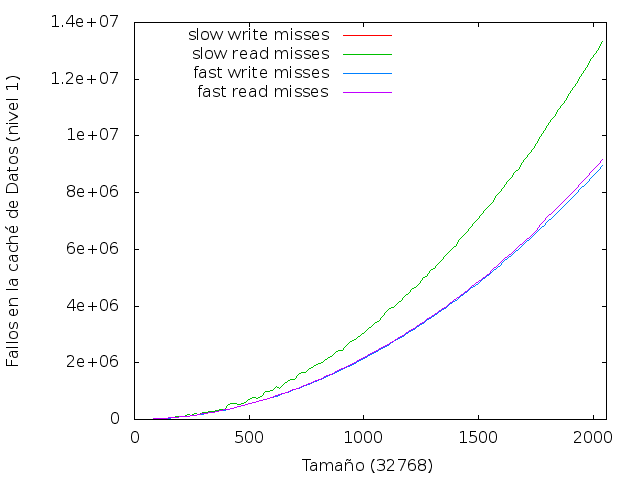
\includegraphics[width=0.8\textwidth]{graficas/fotos/Cache_32768.png}
\end{center}

Esta gráfica ha sido generada con el script de gnuplot \emph{graficas/tamCache\_32768.gp} a partir de los datos almacenados en \emph{data/ej2/tamCache\_32768.dat}

\subsubsection*{8*8192 bytes}
Para una caché de tamaño $P*4*1024$ bytes $= 65536 $ bytes.

\begin{center}
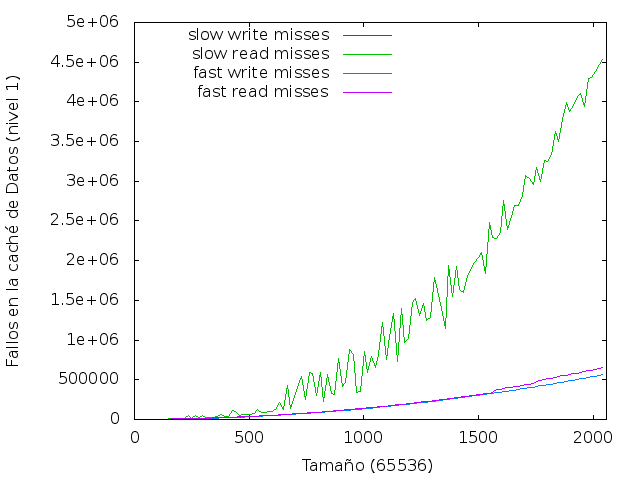
\includegraphics[width=0.8\textwidth]{graficas/fotos/Cache_65536.png}
\end{center}

Esta gráfica ha sido generada con el script de gnuplot \emph{graficas/tamCache\_65536.gp} a partir de los datos almacenados en \emph{data/ej2/tamCache\_65536.dat}


\subsection*{Preguntas}

 \paragraph{¿Se observan cambios de tendencia al variar los tamaños de las cachés?}

Por supuesto, cuanto más grande es la caché menores son los fallos tanto de escritura como de lectura cometidos. Entre las 3 primeras simulaciones no hay una diferencia muy grande. Todas crecen más o menos con la misma rapidez y alcanzan un valor parecido (siempre menor cuanto más grande es la caché), pero viendo la cuarta simulación vemos que los fallos de lectura de \texttt{slow} se reducen casi $\frac{1}{3}$ y los fallos de lectura de \texttt{fast} se aproximan a los de escritura, cambiando incluso su tendencia de crecimiento. Esto es algo bastante lógico, ya que al disponer de cachés de mayor tamaño, podemos almacenar más datos en ellas y por lo tanto reduciremos los fallos.

No podemos deducir nada de la no uniformidad de los fallos de lectura de \texttt{slow}.

\section*{Ejercicio 3}

El código fuente utilizado se encuentra en la carpeta \texttt{src}. Los programas utilizados son \texttt{mult\_norm} para la multiplicación normal y \texttt{mult\_great} para la multiplicación traspuesta (que supusimos que iba a tener mayor rendimiento).

Completamos la ejecución hasta 1300 aproximadamente. Cada ejecución tardaba demasiado y nos hemos quedado sin tiempo para ejecutarla completamente y nuestros compañeros nos han dicho que con 500 era suficiente.

Hemos generado los datos con el script \emph{scripts/genDataMatrix}, que ejecuta los 2 programas y guarda los fallos de lectura, escritura y los tiempos de ejecución de los 2 programas según el tamaño de la matriz.

Toda la información necesaria ha sido almacenada en el fichero \emph{data/ej3/matrix.dat}.

\subsection*{Gr\'aficas}
\subsubsection*{Tiempos de ejecución}
Esta gráfica se ha generado con el script de gnuplot \emph{graficas/multiplies\_times.gp}
\begin{center}
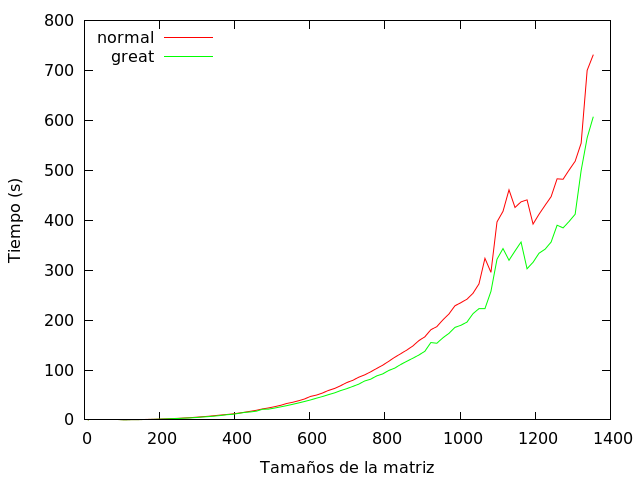
\includegraphics[width=0.8\textwidth]{graficas/fotos/multiplies_times.png}
\end{center}
En esta gráfica pueden observarse picos. Esto se debe a que la ejecución se realizó en una máquina virtual de un ordenador de sobremesa que pudo ser utilizado por alguna otra persona, provocando que el ordenador tuviera momentos de más carga de procesamiento (generado por el sistema operativo anfitrión) y otros momentos en los que el procesador sólo se dedicaba a la simulación en la máquina virtual. A pesar de ello comprobamos que los tiempos de ejecución del programa \texttt{mult\_great} son menores que los del programa \texttt{mult\_norm}. También vemos como va ascendiendo cada vez más ascendiendo a los $800s$, que son aproximadamente 13 minutos.


\subsubsection*{Fallos de escritura}

Esta gráfica se ha generado con el script de gnuplot \emph{"graficas/multiplies\_write.gp"}

\begin{center}
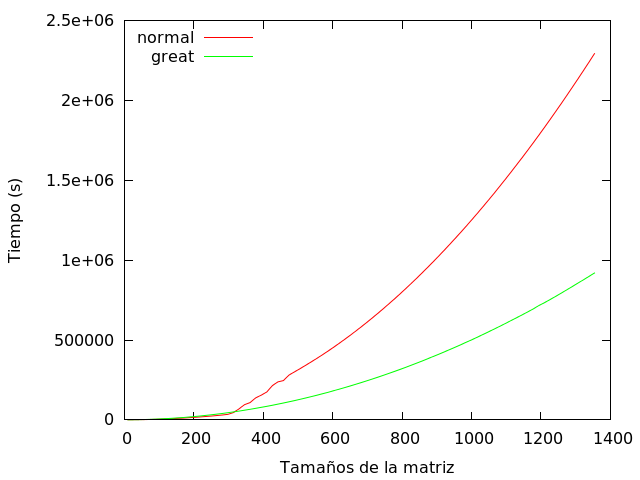
\includegraphics[width=0.8\textwidth]{graficas/fotos/multiplies_write.png}
\end{center}

Podemos comprobar que el programa \texttt{mult\_great} tiene muchos menos fallos de escritura que el \texttt{mult\_norm} (con un tamaño de 1300 son $\displaystyle \frac{2500000}{100000} = 2.5$, un cambio considerable).

\subsubsection*{Fallos de lectura}

Esta gráfica se ha generado con el script de gnuplot \emph{"graficas/multiplies\_read.gp"}

\begin{center}
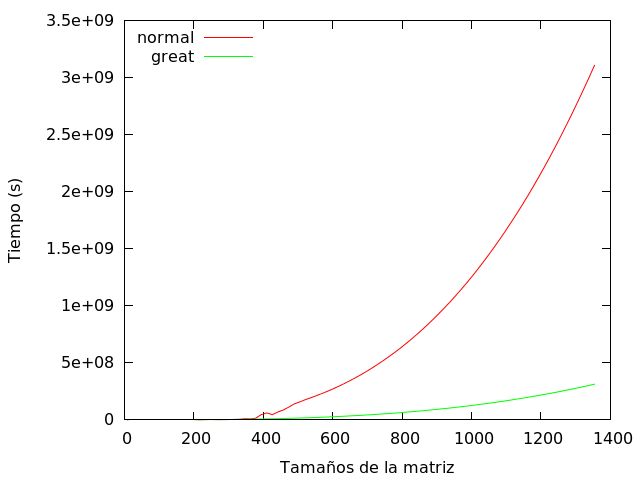
\includegraphics[width=0.8\textwidth]{graficas/fotos/multiplies_read.png}
\end{center}

Lo mismo sucede en este caso con los fallos de lectura.

\subsection*{Preguntas}

\paragraph{¿Se observan cambios en la tendencia al aumentar el tamaño de las matrices?}

Obviamente al aumentar el tamaño de la matriz aumentan los tiempos de ejecución y los fallos de caché (tanto de lectura como de escritura). Además, en la gráfica de fallos de escritura podemos ver cómo, hasta matrices de $300×300$, es más rápido \texttt{mult\_normal}. Sin embargo, la tendencia cambia a partir de ese punto. Puede ocurrir que ese sea el límite en el que la matriz no quepa entera en la caché y por lo tanto cause más fallos de caché. En ese momento, la caché estará continuamente sacando bloques de caché para meter las nuevas filas que se van accediendo continuamente en \texttt{mult\_normal}.

Por otra parte, nuestro código escribe cada celda de la matriz de resultados sólo después de haber calculado el producto de la fila por la columna correspondientes, es decir, se va almacenando de forma temporal en una variable \texttt{sum} y después se guarda en la matriz. Es decir, que la entrada en caché correspondiente en la matriz de resultados apenas se usa, y por lo tanto es más probable que el algoritmo de reemplazo de caché la saque para dar espacio a las filas de los productos.

De esta forma, si se necesita espacio para nuevos bloques de caché porque \texttt{mult\_normal} no accede a las filas de forma ordenada, es más probable que  en cada escritura ocurra un fallo de caché debido a que el bloque de la matriz de resultados no esté. Esto explicaría la diferencia de fallos de escritura entre \texttt{mult\_normal} y \texttt{mult\_great}.

\paragraph{¿Por qué cambia el comportamiento entre la multiplicación normal y la transpuesta?}

Al transponer la matriz, indexamos ambas matrices por filas. Dado que al reservar la memoria cada fila corresponde a un único bloque de memoria, es más probable que en la caché estén las filas contiguas y tengamos menos fallos de caché que al indexar por columnas.

 \end{document}
